% Options for packages loaded elsewhere
\PassOptionsToPackage{unicode}{hyperref}
\PassOptionsToPackage{hyphens}{url}
%
\documentclass[
]{article}
\usepackage{amsmath,amssymb}
\usepackage{iftex}
\ifPDFTeX
  \usepackage[T1]{fontenc}
  \usepackage[utf8]{inputenc}
  \usepackage{textcomp} % provide euro and other symbols
\else % if luatex or xetex
  \usepackage{unicode-math} % this also loads fontspec
  \defaultfontfeatures{Scale=MatchLowercase}
  \defaultfontfeatures[\rmfamily]{Ligatures=TeX,Scale=1}
\fi
\usepackage{lmodern}
\ifPDFTeX\else
  % xetex/luatex font selection
\fi
% Use upquote if available, for straight quotes in verbatim environments
\IfFileExists{upquote.sty}{\usepackage{upquote}}{}
\IfFileExists{microtype.sty}{% use microtype if available
  \usepackage[]{microtype}
  \UseMicrotypeSet[protrusion]{basicmath} % disable protrusion for tt fonts
}{}
\makeatletter
\@ifundefined{KOMAClassName}{% if non-KOMA class
  \IfFileExists{parskip.sty}{%
    \usepackage{parskip}
  }{% else
    \setlength{\parindent}{0pt}
    \setlength{\parskip}{6pt plus 2pt minus 1pt}}
}{% if KOMA class
  \KOMAoptions{parskip=half}}
\makeatother
\usepackage{xcolor}
\usepackage[margin=1in]{geometry}
\usepackage{color}
\usepackage{fancyvrb}
\newcommand{\VerbBar}{|}
\newcommand{\VERB}{\Verb[commandchars=\\\{\}]}
\DefineVerbatimEnvironment{Highlighting}{Verbatim}{commandchars=\\\{\}}
% Add ',fontsize=\small' for more characters per line
\usepackage{framed}
\definecolor{shadecolor}{RGB}{248,248,248}
\newenvironment{Shaded}{\begin{snugshade}}{\end{snugshade}}
\newcommand{\AlertTok}[1]{\textcolor[rgb]{0.94,0.16,0.16}{#1}}
\newcommand{\AnnotationTok}[1]{\textcolor[rgb]{0.56,0.35,0.01}{\textbf{\textit{#1}}}}
\newcommand{\AttributeTok}[1]{\textcolor[rgb]{0.13,0.29,0.53}{#1}}
\newcommand{\BaseNTok}[1]{\textcolor[rgb]{0.00,0.00,0.81}{#1}}
\newcommand{\BuiltInTok}[1]{#1}
\newcommand{\CharTok}[1]{\textcolor[rgb]{0.31,0.60,0.02}{#1}}
\newcommand{\CommentTok}[1]{\textcolor[rgb]{0.56,0.35,0.01}{\textit{#1}}}
\newcommand{\CommentVarTok}[1]{\textcolor[rgb]{0.56,0.35,0.01}{\textbf{\textit{#1}}}}
\newcommand{\ConstantTok}[1]{\textcolor[rgb]{0.56,0.35,0.01}{#1}}
\newcommand{\ControlFlowTok}[1]{\textcolor[rgb]{0.13,0.29,0.53}{\textbf{#1}}}
\newcommand{\DataTypeTok}[1]{\textcolor[rgb]{0.13,0.29,0.53}{#1}}
\newcommand{\DecValTok}[1]{\textcolor[rgb]{0.00,0.00,0.81}{#1}}
\newcommand{\DocumentationTok}[1]{\textcolor[rgb]{0.56,0.35,0.01}{\textbf{\textit{#1}}}}
\newcommand{\ErrorTok}[1]{\textcolor[rgb]{0.64,0.00,0.00}{\textbf{#1}}}
\newcommand{\ExtensionTok}[1]{#1}
\newcommand{\FloatTok}[1]{\textcolor[rgb]{0.00,0.00,0.81}{#1}}
\newcommand{\FunctionTok}[1]{\textcolor[rgb]{0.13,0.29,0.53}{\textbf{#1}}}
\newcommand{\ImportTok}[1]{#1}
\newcommand{\InformationTok}[1]{\textcolor[rgb]{0.56,0.35,0.01}{\textbf{\textit{#1}}}}
\newcommand{\KeywordTok}[1]{\textcolor[rgb]{0.13,0.29,0.53}{\textbf{#1}}}
\newcommand{\NormalTok}[1]{#1}
\newcommand{\OperatorTok}[1]{\textcolor[rgb]{0.81,0.36,0.00}{\textbf{#1}}}
\newcommand{\OtherTok}[1]{\textcolor[rgb]{0.56,0.35,0.01}{#1}}
\newcommand{\PreprocessorTok}[1]{\textcolor[rgb]{0.56,0.35,0.01}{\textit{#1}}}
\newcommand{\RegionMarkerTok}[1]{#1}
\newcommand{\SpecialCharTok}[1]{\textcolor[rgb]{0.81,0.36,0.00}{\textbf{#1}}}
\newcommand{\SpecialStringTok}[1]{\textcolor[rgb]{0.31,0.60,0.02}{#1}}
\newcommand{\StringTok}[1]{\textcolor[rgb]{0.31,0.60,0.02}{#1}}
\newcommand{\VariableTok}[1]{\textcolor[rgb]{0.00,0.00,0.00}{#1}}
\newcommand{\VerbatimStringTok}[1]{\textcolor[rgb]{0.31,0.60,0.02}{#1}}
\newcommand{\WarningTok}[1]{\textcolor[rgb]{0.56,0.35,0.01}{\textbf{\textit{#1}}}}
\usepackage{graphicx}
\makeatletter
\def\maxwidth{\ifdim\Gin@nat@width>\linewidth\linewidth\else\Gin@nat@width\fi}
\def\maxheight{\ifdim\Gin@nat@height>\textheight\textheight\else\Gin@nat@height\fi}
\makeatother
% Scale images if necessary, so that they will not overflow the page
% margins by default, and it is still possible to overwrite the defaults
% using explicit options in \includegraphics[width, height, ...]{}
\setkeys{Gin}{width=\maxwidth,height=\maxheight,keepaspectratio}
% Set default figure placement to htbp
\makeatletter
\def\fps@figure{htbp}
\makeatother
\setlength{\emergencystretch}{3em} % prevent overfull lines
\providecommand{\tightlist}{%
  \setlength{\itemsep}{0pt}\setlength{\parskip}{0pt}}
\setcounter{secnumdepth}{-\maxdimen} % remove section numbering
% definitions for citeproc citations
\NewDocumentCommand\citeproctext{}{}
\NewDocumentCommand\citeproc{mm}{%
  \begingroup\def\citeproctext{#2}\cite{#1}\endgroup}
\makeatletter
 % allow citations to break across lines
 \let\@cite@ofmt\@firstofone
 % avoid brackets around text for \cite:
 \def\@biblabel#1{}
 \def\@cite#1#2{{#1\if@tempswa , #2\fi}}
\makeatother
\newlength{\cslhangindent}
\setlength{\cslhangindent}{1.5em}
\newlength{\csllabelwidth}
\setlength{\csllabelwidth}{3em}
\newenvironment{CSLReferences}[2] % #1 hanging-indent, #2 entry-spacing
 {\begin{list}{}{%
  \setlength{\itemindent}{0pt}
  \setlength{\leftmargin}{0pt}
  \setlength{\parsep}{0pt}
  % turn on hanging indent if param 1 is 1
  \ifodd #1
   \setlength{\leftmargin}{\cslhangindent}
   \setlength{\itemindent}{-1\cslhangindent}
  \fi
  % set entry spacing
  \setlength{\itemsep}{#2\baselineskip}}}
 {\end{list}}
\usepackage{calc}
\newcommand{\CSLBlock}[1]{\hfill\break\parbox[t]{\linewidth}{\strut\ignorespaces#1\strut}}
\newcommand{\CSLLeftMargin}[1]{\parbox[t]{\csllabelwidth}{\strut#1\strut}}
\newcommand{\CSLRightInline}[1]{\parbox[t]{\linewidth - \csllabelwidth}{\strut#1\strut}}
\newcommand{\CSLIndent}[1]{\hspace{\cslhangindent}#1}
\ifLuaTeX
  \usepackage{selnolig}  % disable illegal ligatures
\fi
\usepackage{bookmark}
\IfFileExists{xurl.sty}{\usepackage{xurl}}{} % add URL line breaks if available
\urlstyle{same}
\hypersetup{
  pdftitle={Proyecto\_RNAseq},
  pdfauthor={Karla Ximena González Platas},
  hidelinks,
  pdfcreator={LaTeX via pandoc}}

\title{Proyecto\_RNAseq}
\usepackage{etoolbox}
\makeatletter
\providecommand{\subtitle}[1]{% add subtitle to \maketitle
  \apptocmd{\@title}{\par {\large #1 \par}}{}{}
}
\makeatother
\subtitle{Análisis de Expresión Diferencial}
\author{Karla Ximena González Platas}
\date{2025-02-05}

\begin{document}
\maketitle

{
\setcounter{tocdepth}{2}
\tableofcontents
}
\subsection{Introducción}\label{introducciuxf3n}

El conjunto de datos analizado en este proyecto se deriva del estudio de
Muluhngwi y Klinge (2021), que explora las interacciones regulatorias
entre los miembros de la familia miR-29 y los lncRNAs (ARN largos no
codificantes) en el contexto de la resistencia a la terapia endocrina.
En este estudio, se aplicó el análisis de RNA-seq para investigar la
expresión de lncRNAs regulados por miR-29b-1-3p y miR-29a-3p en células
de cáncer de mama sensibles a la terapia endocrina (MCF-7) y resistentes
a la terapia endocrina (LCC9). Estas líneas celulares fueron empleadas
para estudiar los efectos de la regulación de lncRNAs por los
miR-29b-1-3p y miR-29a-3p en la resistencia endocrina del cáncer de
mama. Para ello, se realizaron transfecciones en las células MCF-7 y
LCC9 con pre-miR-29b-1-3p y pre-miR-29a-3p para evaluar los efectos de
su sobreexpresión en la proliferación celular y en la regulación de
lncRNAs. Mientras tanto, el uso de anti-miR-29 y un control negativo
permitió analizar la inhibición de estos miRNAs.(Muluhngwi and Klinge
2021)

\subsection{Pregunta de
investigación}\label{pregunta-de-investigaciuxf3n}

¿Cuáles son los genes diferencialmente expresados entre las células de
cáncer de mama sensibles (MCF-7) y resistentes (LCC9) a la terapia
endocrina, y cómo se ven afectados por la sobreexpresión e inhibición de
miR-29a y miR-29b-1?

\subsection{Hipótesis}\label{hipuxf3tesis}

La sobreexpresión de miR-29a y miR-29b-1 en las células de cáncer de
mama sensibles (MCF-7) y resistentes (LCC9) a la terapia endocrina
altera la expresión de genes involucrados en la resistencia a los
tratamientos.

\subsection{Instalación y carga de
paquetes}\label{instalaciuxf3n-y-carga-de-paquetes}

\begin{Shaded}
\begin{Highlighting}[]
\CommentTok{\# Instalar BiocManager si no está instalado}
\CommentTok{\#if (!requireNamespace("BiocManager", quietly = TRUE)) \{}
\CommentTok{\#    install.packages("BiocManager")}
\CommentTok{\#\}}

\CommentTok{\# Instalar paquetes de Bioconductor}
\CommentTok{\#BiocManager::install(}
\CommentTok{\#    c(}
\CommentTok{\#        "edgeR", }
\CommentTok{\#        "ExploreModelMatrix",}
\CommentTok{\#        "limma",}
\CommentTok{\#        "recount3", }
\CommentTok{\#        "SummarizedExperiment", }
\CommentTok{\#        "GenomicRanges"}
\CommentTok{\#    )}
\CommentTok{\#)}

\CommentTok{\# Instalar paquetes de CRAN}
\CommentTok{\#install.packages(c(}
\CommentTok{\#    "pheatmap", }
\CommentTok{\#    "patchwork",}
\CommentTok{\#    "RColorBrewer",}
\CommentTok{\#    "cowplot"}
\CommentTok{\#))}

\DocumentationTok{\#\# Cargar los paquetes}
\FunctionTok{library}\NormalTok{(}\StringTok{"recount3"}\NormalTok{)}
\FunctionTok{library}\NormalTok{(}\StringTok{"SummarizedExperiment"}\NormalTok{)}
\FunctionTok{library}\NormalTok{(}\StringTok{"GenomicRanges"}\NormalTok{)}
\FunctionTok{library}\NormalTok{(}\StringTok{"limma"}\NormalTok{)}
\FunctionTok{library}\NormalTok{(}\StringTok{"edgeR"}\NormalTok{)}
\FunctionTok{library}\NormalTok{(}\StringTok{"ExploreModelMatrix"}\NormalTok{)}
\FunctionTok{library}\NormalTok{(}\StringTok{"cowplot"}\NormalTok{)}
\FunctionTok{library}\NormalTok{(}\StringTok{"RColorBrewer"}\NormalTok{)}
\FunctionTok{library}\NormalTok{(}\StringTok{"pheatmap"}\NormalTok{)}
\end{Highlighting}
\end{Shaded}

\subsection{Selección de Proyecto}\label{selecciuxf3n-de-proyecto}

\begin{Shaded}
\begin{Highlighting}[]
\CommentTok{\# Obtener la lista de proyectos disponibles }
\NormalTok{human\_projects }\OtherTok{\textless{}{-}} \FunctionTok{available\_projects}\NormalTok{()}
\end{Highlighting}
\end{Shaded}

\begin{verbatim}
## 2025-02-08 00:18:49.0854 caching file sra.recount_project.MD.gz.
\end{verbatim}

\begin{verbatim}
## 2025-02-08 00:18:50.896875 caching file gtex.recount_project.MD.gz.
\end{verbatim}

\begin{verbatim}
## 2025-02-08 00:18:51.650773 caching file tcga.recount_project.MD.gz.
\end{verbatim}

\begin{Shaded}
\begin{Highlighting}[]
\CommentTok{\# Ver los proyectos disponibles}
\FunctionTok{dim}\NormalTok{(human\_projects)}
\end{Highlighting}
\end{Shaded}

\begin{verbatim}
## [1] 8742    6
\end{verbatim}

\begin{Shaded}
\begin{Highlighting}[]
\CommentTok{\# Esto nos indica cuántos proyectos están disponibles (número de filas) }
\CommentTok{\# y cuántas columnas de información se proporcionan para cada proyecto.}

\CommentTok{\# Mostrar las primeras filas para inspeccionar su estructura y contenido}
\FunctionTok{head}\NormalTok{(human\_projects)}
\end{Highlighting}
\end{Shaded}

\begin{verbatim}
##     project organism file_source     project_home project_type n_samples
## 1 SRP107565    human         sra data_sources/sra data_sources       216
## 2 SRP149665    human         sra data_sources/sra data_sources         4
## 3 SRP017465    human         sra data_sources/sra data_sources        23
## 4 SRP119165    human         sra data_sources/sra data_sources         6
## 5 SRP133965    human         sra data_sources/sra data_sources        12
## 6 SRP096765    human         sra data_sources/sra data_sources         7
\end{verbatim}

\begin{Shaded}
\begin{Highlighting}[]
\CommentTok{\# Seleccionar un estudio de interés}
\NormalTok{human\_projects[}\DecValTok{709}\NormalTok{, ]}
\end{Highlighting}
\end{Shaded}

\begin{verbatim}
##       project organism file_source     project_home project_type n_samples
## 709 SRP075398    human         sra data_sources/sra data_sources        18
\end{verbatim}

\begin{Shaded}
\begin{Highlighting}[]
\CommentTok{\# Filtrar el dataframe para seleccionar un proyecto específico basado en su ID y tipo}
\NormalTok{project\_info }\OtherTok{\textless{}{-}} \FunctionTok{subset}\NormalTok{(}
\NormalTok{  human\_projects,}
\NormalTok{  project }\SpecialCharTok{==} \StringTok{"SRP075398"} \SpecialCharTok{\&}\NormalTok{ project\_type }\SpecialCharTok{==} \StringTok{"data\_sources"}
\NormalTok{)}

\CommentTok{\# Mostrar la información del proyecto seleccionado para confirmar que se ha}
\CommentTok{\# filtrado correctamente}
\NormalTok{project\_info}
\end{Highlighting}
\end{Shaded}

\begin{verbatim}
##       project organism file_source     project_home project_type n_samples
## 709 SRP075398    human         sra data_sources/sra data_sources        18
\end{verbatim}

\begin{Shaded}
\begin{Highlighting}[]
\CommentTok{\# Crear un objeto de tipo RangedSummarizedExperiment (RSE) con la información}
\CommentTok{\# a nivel de genes}
\NormalTok{rse\_gene\_SRP075398 }\OtherTok{\textless{}{-}} \FunctionTok{create\_rse}\NormalTok{(project\_info)}
\end{Highlighting}
\end{Shaded}

\begin{verbatim}
## 2025-02-08 00:19:00.25997 downloading and reading the metadata.
\end{verbatim}

\begin{verbatim}
## 2025-02-08 00:19:01.369594 caching file sra.sra.SRP075398.MD.gz.
\end{verbatim}

\begin{verbatim}
## 2025-02-08 00:19:02.226195 caching file sra.recount_project.SRP075398.MD.gz.
\end{verbatim}

\begin{verbatim}
## 2025-02-08 00:19:03.050879 caching file sra.recount_qc.SRP075398.MD.gz.
\end{verbatim}

\begin{verbatim}
## 2025-02-08 00:19:03.900093 caching file sra.recount_seq_qc.SRP075398.MD.gz.
\end{verbatim}

\begin{verbatim}
## 2025-02-08 00:19:04.795734 caching file sra.recount_pred.SRP075398.MD.gz.
\end{verbatim}

\begin{verbatim}
## 2025-02-08 00:19:05.043538 downloading and reading the feature information.
\end{verbatim}

\begin{verbatim}
## 2025-02-08 00:19:05.604873 caching file human.gene_sums.G026.gtf.gz.
\end{verbatim}

\begin{verbatim}
## 2025-02-08 00:19:06.663228 downloading and reading the counts: 18 samples across 63856 features.
\end{verbatim}

\begin{verbatim}
## 2025-02-08 00:19:07.348284 caching file sra.gene_sums.SRP075398.G026.gz.
\end{verbatim}

\begin{verbatim}
## 2025-02-08 00:19:07.91128 constructing the RangedSummarizedExperiment (rse) object.
\end{verbatim}

\begin{Shaded}
\begin{Highlighting}[]
\CommentTok{\# Explorar el objeto RSE}
\NormalTok{rse\_gene\_SRP075398}
\end{Highlighting}
\end{Shaded}

\begin{verbatim}
## class: RangedSummarizedExperiment 
## dim: 63856 18 
## metadata(8): time_created recount3_version ... annotation recount3_url
## assays(1): raw_counts
## rownames(63856): ENSG00000278704.1 ENSG00000277400.1 ...
##   ENSG00000182484.15_PAR_Y ENSG00000227159.8_PAR_Y
## rowData names(10): source type ... havana_gene tag
## colnames(18): SRR3544525 SRR3544526 ... SRR3544537 SRR3544540
## colData names(175): rail_id external_id ...
##   recount_pred.curated.cell_line BigWigURL
\end{verbatim}

\begin{Shaded}
\begin{Highlighting}[]
\DocumentationTok{\#\# Información sobre el RSE creado}
\FunctionTok{metadata}\NormalTok{(rse\_gene\_SRP075398)}
\end{Highlighting}
\end{Shaded}

\begin{verbatim}
## $time_created
## [1] "2025-02-08 00:19:07 CST"
## 
## $recount3_version
##           package ondiskversion loadedversion
## recount3 recount3        1.16.0        1.16.0
##                                            path
## recount3 /usr/local/lib/R/site-library/recount3
##                                      loadedpath attached is_base       date
## recount3 /usr/local/lib/R/site-library/recount3     TRUE   FALSE 2024-10-29
##                               source md5ok                       library
## recount3 Bioconductor 3.20 (R 4.4.2)    NA /usr/local/lib/R/site-library
## 
## $project
## [1] "SRP075398"
## 
## $project_home
## [1] "data_sources/sra"
## 
## $type
## [1] "gene"
## 
## $organism
## [1] "human"
## 
## $annotation
## [1] "gencode_v26"
## 
## $recount3_url
## [1] "http://duffel.rail.bio/recount3"
\end{verbatim}

\begin{Shaded}
\begin{Highlighting}[]
\DocumentationTok{\#\# Número de genes y número de muestras}
\FunctionTok{dim}\NormalTok{(rse\_gene\_SRP075398)}
\end{Highlighting}
\end{Shaded}

\begin{verbatim}
## [1] 63856    18
\end{verbatim}

El estudio \textbf{SRP075398} se compuso de \textbf{18 muestras}, para
las cuales tenemos \textbf{63,856 genes} en GENCODE v26. La información
específica de la anotación está disponible rowRanges() como se muestra a
continuación con la columna gene\_id utilizada para identificar genes en
cada una de las anotaciones.

\begin{Shaded}
\begin{Highlighting}[]
\CommentTok{\# Información sobre los genes}
\FunctionTok{rowRanges}\NormalTok{(rse\_gene\_SRP075398)}
\end{Highlighting}
\end{Shaded}

\begin{verbatim}
## GRanges object with 63856 ranges and 10 metadata columns:
##                              seqnames            ranges strand |   source
##                                 <Rle>         <IRanges>  <Rle> | <factor>
##          ENSG00000278704.1 GL000009.2       56140-58376      - |  ENSEMBL
##          ENSG00000277400.1 GL000194.1      53590-115018      - |  ENSEMBL
##          ENSG00000274847.1 GL000194.1      53594-115055      - |  ENSEMBL
##          ENSG00000277428.1 GL000195.1       37434-37534      - |  ENSEMBL
##          ENSG00000276256.1 GL000195.1       42939-49164      - |  ENSEMBL
##                        ...        ...               ...    ... .      ...
##   ENSG00000124334.17_PAR_Y       chrY 57184101-57197337      + |   HAVANA
##   ENSG00000185203.12_PAR_Y       chrY 57201143-57203357      - |   HAVANA
##    ENSG00000270726.6_PAR_Y       chrY 57190738-57208756      + |   HAVANA
##   ENSG00000182484.15_PAR_Y       chrY 57207346-57212230      + |   HAVANA
##    ENSG00000227159.8_PAR_Y       chrY 57212184-57214397      - |   HAVANA
##                                type bp_length     phase                gene_id
##                            <factor> <numeric> <integer>            <character>
##          ENSG00000278704.1     gene      2237      <NA>      ENSG00000278704.1
##          ENSG00000277400.1     gene      2179      <NA>      ENSG00000277400.1
##          ENSG00000274847.1     gene      1599      <NA>      ENSG00000274847.1
##          ENSG00000277428.1     gene       101      <NA>      ENSG00000277428.1
##          ENSG00000276256.1     gene      2195      <NA>      ENSG00000276256.1
##                        ...      ...       ...       ...                    ...
##   ENSG00000124334.17_PAR_Y     gene      2504      <NA> ENSG00000124334.17_P..
##   ENSG00000185203.12_PAR_Y     gene      1054      <NA> ENSG00000185203.12_P..
##    ENSG00000270726.6_PAR_Y     gene       773      <NA> ENSG00000270726.6_PA..
##   ENSG00000182484.15_PAR_Y     gene      4618      <NA> ENSG00000182484.15_P..
##    ENSG00000227159.8_PAR_Y     gene      1306      <NA> ENSG00000227159.8_PA..
##                                         gene_type   gene_name       level
##                                       <character> <character> <character>
##          ENSG00000278704.1         protein_coding  BX004987.1           3
##          ENSG00000277400.1         protein_coding  AC145212.2           3
##          ENSG00000274847.1         protein_coding  AC145212.1           3
##          ENSG00000277428.1               misc_RNA       Y_RNA           3
##          ENSG00000276256.1         protein_coding  AC011043.1           3
##                        ...                    ...         ...         ...
##   ENSG00000124334.17_PAR_Y         protein_coding        IL9R           2
##   ENSG00000185203.12_PAR_Y              antisense      WASIR1           2
##    ENSG00000270726.6_PAR_Y   processed_transcript AJ271736.10           2
##   ENSG00000182484.15_PAR_Y transcribed_unproces..      WASH6P           2
##    ENSG00000227159.8_PAR_Y unprocessed_pseudogene    DDX11L16           2
##                                     havana_gene         tag
##                                     <character> <character>
##          ENSG00000278704.1                 <NA>        <NA>
##          ENSG00000277400.1                 <NA>        <NA>
##          ENSG00000274847.1                 <NA>        <NA>
##          ENSG00000277428.1                 <NA>        <NA>
##          ENSG00000276256.1                 <NA>        <NA>
##                        ...                  ...         ...
##   ENSG00000124334.17_PAR_Y OTTHUMG00000022720.1         PAR
##   ENSG00000185203.12_PAR_Y OTTHUMG00000022676.3         PAR
##    ENSG00000270726.6_PAR_Y OTTHUMG00000184987.2         PAR
##   ENSG00000182484.15_PAR_Y OTTHUMG00000022677.5         PAR
##    ENSG00000227159.8_PAR_Y OTTHUMG00000022678.1         PAR
##   -------
##   seqinfo: 374 sequences from an unspecified genome; no seqlengths
\end{verbatim}

\subsection{Preparación de los datos}\label{preparaciuxf3n-de-los-datos}

\begin{Shaded}
\begin{Highlighting}[]
\CommentTok{\# Convertir las cuentas por nucleotido a cuentas por lectura usando compute\_read\_counts()}
\FunctionTok{assay}\NormalTok{(rse\_gene\_SRP075398, }\StringTok{"counts"}\NormalTok{) }\OtherTok{\textless{}{-}} \FunctionTok{compute\_read\_counts}\NormalTok{(rse\_gene\_SRP075398)}

\CommentTok{\# Inspeccionar la información experimental de cada muestra}
\NormalTok{rse\_gene\_SRP075398}\SpecialCharTok{$}\NormalTok{sra.sample\_attributes[]}
\end{Highlighting}
\end{Shaded}

\begin{verbatim}
##  [1] "cell line;;LCC9|source_name;;LCC9 cell line pre-miR-29b-1 transfected|transfection;;Pre-miR-29b-1"  
##  [2] "cell line;;LCC9|source_name;;LCC9 cell line Anti-miR-29a transfected|transfection;;Anti-miR-29a"    
##  [3] "cell line;;LCC9|source_name;;LCC9 cell line Anti-miR-29a transfected|transfection;;Anti-miR-29a"    
##  [4] "cell line;;LCC9|source_name;;LCC9 cell line Anti-miR-29a transfected|transfection;;Anti-miR-29a"    
##  [5] "cell line;;LCC9|source_name;;LCC9 cell line Pre-miR-29a transfected|transfection;;Pre-miR-29a"      
##  [6] "cell line;;LCC9|source_name;;LCC9 cell line Pre-miR-29a transfected|transfection;;Pre-miR-29a"      
##  [7] "cell line;;LCC9|source_name;;LCC9 cell line Pre-miR-29a transfected|transfection;;Pre-miR-29a"      
##  [8] "cell line;;MCF-7|source_name;;MCF-7 cell line pre-miR-29b-1 transfected|transfection;;Pre-miR-29b-1"
##  [9] "cell line;;MCF-7|source_name;;MCF-7 cell line pre-miR-29b-1 transfected|transfection;;Pre-miR-29b-1"
## [10] "cell line;;MCF-7|source_name;;MCF-7 cell line Pre-miR-29a transfected|transfection;;Pre-miR-29a"    
## [11] "cell line;;MCF-7|source_name;;MCF-7 cell line Pre-miR-29a transfected|transfection;;Pre-miR-29a"    
## [12] "cell line;;LCC9|source_name;;LCC9 cell line pre-miR-29b-1 transfected|transfection;;Pre-miR-29b-1"  
## [13] "cell line;;LCC9|source_name;;LCC9 cell line pre-miR-29b-1 transfected|transfection;;Pre-miR-29b-1"  
## [14] "cell line;;MCF-7|source_name;;MCF-7 cell line pre-miR-29b-1 transfected|transfection;;Pre-miR-29b-1"
## [15] "cell line;;MCF-7|source_name;;MCF-7 cell line Anti-miR-29a transfected|transfection;;Anti-miR-29a"  
## [16] "cell line;;MCF-7|source_name;;MCF-7 cell line Anti-miR-29a transfected|transfection;;Anti-miR-29a"  
## [17] "cell line;;MCF-7|source_name;;MCF-7 cell line Anti-miR-29a transfected|transfection;;Anti-miR-29a"  
## [18] "cell line;;MCF-7|source_name;;MCF-7 cell line Pre-miR-29a transfected|transfection;;Pre-miR-29a"
\end{verbatim}

\begin{Shaded}
\begin{Highlighting}[]
\CommentTok{\# Expandir los atributos en columnas separadas para facilitar su uso}
\NormalTok{rse\_gene\_SRP075398 }\OtherTok{\textless{}{-}} \FunctionTok{expand\_sra\_attributes}\NormalTok{(rse\_gene\_SRP075398)}

\CommentTok{\# Extraer y mostrar las columnas que contienen atributos }
\FunctionTok{colData}\NormalTok{(rse\_gene\_SRP075398)[}
\NormalTok{  ,}
  \FunctionTok{grepl}\NormalTok{(}\StringTok{"\^{}sra\_attribute"}\NormalTok{, }\FunctionTok{colnames}\NormalTok{(}\FunctionTok{colData}\NormalTok{(rse\_gene\_SRP075398)))}
\NormalTok{]}
\end{Highlighting}
\end{Shaded}

\begin{verbatim}
## DataFrame with 18 rows and 3 columns
##            sra_attribute.cell_line sra_attribute.source_name
##                        <character>               <character>
## SRR3544525                    LCC9    LCC9 cell line pre-m..
## SRR3544526                    LCC9    LCC9 cell line Anti-..
## SRR3544527                    LCC9    LCC9 cell line Anti-..
## SRR3544528                    LCC9    LCC9 cell line Anti-..
## SRR3544529                    LCC9    LCC9 cell line Pre-m..
## ...                            ...                       ...
## SRR3544534                   MCF-7    MCF-7 cell line pre-..
## SRR3544535                   MCF-7    MCF-7 cell line Anti..
## SRR3544536                   MCF-7    MCF-7 cell line Anti..
## SRR3544537                   MCF-7    MCF-7 cell line Anti..
## SRR3544540                   MCF-7    MCF-7 cell line Pre-..
##            sra_attribute.transfection
##                           <character>
## SRR3544525              Pre-miR-29b-1
## SRR3544526               Anti-miR-29a
## SRR3544527               Anti-miR-29a
## SRR3544528               Anti-miR-29a
## SRR3544529                Pre-miR-29a
## ...                               ...
## SRR3544534              Pre-miR-29b-1
## SRR3544535               Anti-miR-29a
## SRR3544536               Anti-miR-29a
## SRR3544537               Anti-miR-29a
## SRR3544540                Pre-miR-29a
\end{verbatim}

\begin{Shaded}
\begin{Highlighting}[]
\CommentTok{\# Ajustar el tipo de dato de las variables categóricas }

\NormalTok{rse\_gene\_SRP075398}\SpecialCharTok{$}\NormalTok{sra\_attribute.cell\_line }\OtherTok{\textless{}{-}} 
  \FunctionTok{factor}\NormalTok{(rse\_gene\_SRP075398}\SpecialCharTok{$}\NormalTok{sra\_attribute.cell\_line)}

\NormalTok{rse\_gene\_SRP075398}\SpecialCharTok{$}\NormalTok{sra\_attribute.source\_name }\OtherTok{\textless{}{-}} 
  \FunctionTok{factor}\NormalTok{(}\FunctionTok{tolower}\NormalTok{(rse\_gene\_SRP075398}\SpecialCharTok{$}\NormalTok{sra\_attribute.source\_name))}

\NormalTok{rse\_gene\_SRP075398}\SpecialCharTok{$}\NormalTok{sra\_attribute.transfection }\OtherTok{\textless{}{-}}   
  \FunctionTok{factor}\NormalTok{(rse\_gene\_SRP075398}\SpecialCharTok{$}\NormalTok{sra\_attribute.transfection)}

\CommentTok{\# Resumen estadístico de las variables seleccionadas}
\FunctionTok{summary}\NormalTok{(}\FunctionTok{as.data.frame}\NormalTok{(}\FunctionTok{colData}\NormalTok{(rse\_gene\_SRP075398)[}
\NormalTok{    ,}
    \FunctionTok{grepl}\NormalTok{(}\StringTok{"\^{}sra\_attribute.[cell\_line|source\_name|transfection]"}\NormalTok{, }
          \FunctionTok{colnames}\NormalTok{(}\FunctionTok{colData}\NormalTok{(rse\_gene\_SRP075398)))}
\NormalTok{    ]))}
\end{Highlighting}
\end{Shaded}

\begin{verbatim}
##  sra_attribute.cell_line                             sra_attribute.source_name
##  LCC9 :9                 lcc9 cell line anti-mir-29a transfected  :3          
##  MCF-7:9                 lcc9 cell line pre-mir-29a transfected   :3          
##                          lcc9 cell line pre-mir-29b-1 transfected :3          
##                          mcf-7 cell line anti-mir-29a transfected :3          
##                          mcf-7 cell line pre-mir-29a transfected  :3          
##                          mcf-7 cell line pre-mir-29b-1 transfected:3          
##  sra_attribute.transfection
##  Anti-miR-29a :6           
##  Pre-miR-29a  :6           
##  Pre-miR-29b-1:6           
##                            
##                            
## 
\end{verbatim}

\begin{Shaded}
\begin{Highlighting}[]
\CommentTok{\# Calcular la proporción de lecturas asignadas a genes para evaluar la calidad}
\CommentTok{\# de las muestras}

\NormalTok{rse\_gene\_SRP075398}\SpecialCharTok{$}\NormalTok{assigned\_gene\_prop }\OtherTok{\textless{}{-}} 
\NormalTok{  rse\_gene\_SRP075398}\SpecialCharTok{$}\NormalTok{recount\_qc.gene\_fc\_count\_all.assigned }\SpecialCharTok{/} 
\NormalTok{  rse\_gene\_SRP075398}\SpecialCharTok{$}\NormalTok{recount\_qc.gene\_fc\_count\_all.total}

\CommentTok{\# Resumen de la nueva variable para identificar si las muestras tienen una }
\CommentTok{\# asignación adecuada de lecturas (valores cercanos a 1 son indicadores de buena calidad)}

\FunctionTok{summary}\NormalTok{(rse\_gene\_SRP075398}\SpecialCharTok{$}\NormalTok{assigned\_gene\_prop)}
\end{Highlighting}
\end{Shaded}

\begin{verbatim}
##    Min. 1st Qu.  Median    Mean 3rd Qu.    Max. 
##  0.6076  0.6405  0.6603  0.6585  0.6696  0.7017
\end{verbatim}

\subsection{Filtrar genes de baja
expresión}\label{filtrar-genes-de-baja-expresiuxf3n}

\begin{Shaded}
\begin{Highlighting}[]
\CommentTok{\# Guardar el objeto original}
\NormalTok{rse\_gene\_SRP075398\_unfiltered }\OtherTok{\textless{}{-}}\NormalTok{ rse\_gene\_SRP075398}

\CommentTok{\# Visualizar la distribución de la proporción de lecturas asignadas a genes en}
\CommentTok{\# cada muestra}

\FunctionTok{hist}\NormalTok{(rse\_gene\_SRP075398}\SpecialCharTok{$}\NormalTok{assigned\_gene\_prop, }
     \AttributeTok{main =} \StringTok{"Proporción de lecturas asignadas a genes"}\NormalTok{, }
     \AttributeTok{xlab =} \StringTok{"Proporción asignada"}\NormalTok{, }\AttributeTok{col =} \StringTok{"lightblue"}\NormalTok{)}
\end{Highlighting}
\end{Shaded}

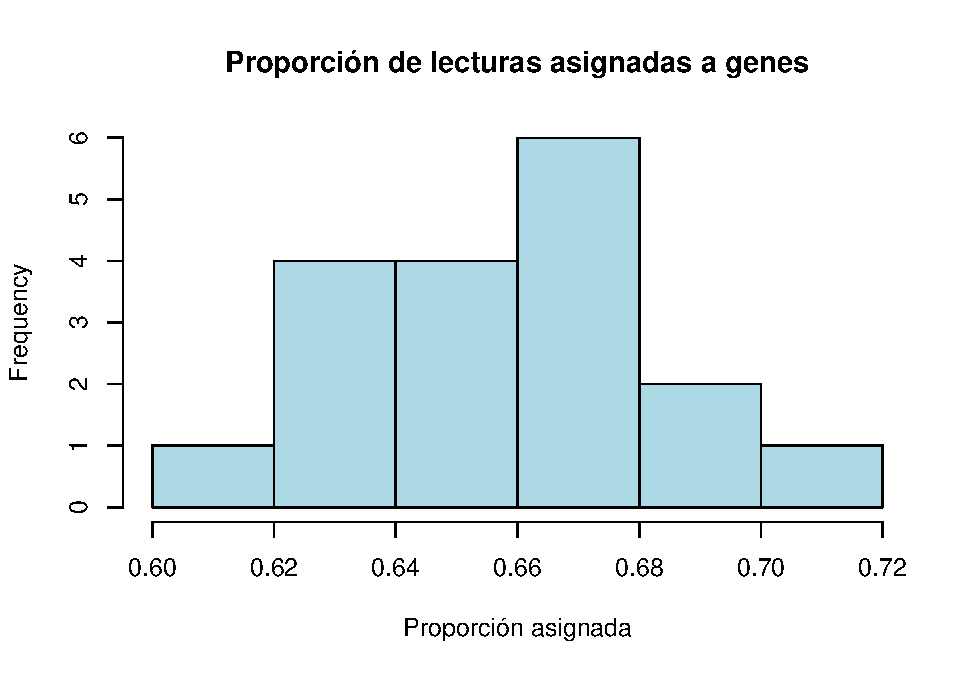
\includegraphics{Proyecto_RNAseq_files/figure-latex/unnamed-chunk-8-1.pdf}

\begin{Shaded}
\begin{Highlighting}[]
\CommentTok{\# Verificar si existen muestras de baja calidad antes del filtrado}
\FunctionTok{table}\NormalTok{(rse\_gene\_SRP075398}\SpecialCharTok{$}\NormalTok{assigned\_gene\_prop }\SpecialCharTok{\textless{}} \FloatTok{0.3}\NormalTok{)}
\end{Highlighting}
\end{Shaded}

\begin{verbatim}
## 
## FALSE 
##    18
\end{verbatim}

\begin{Shaded}
\begin{Highlighting}[]
\CommentTok{\# Filtrar las muestras con proporción de lecturas asignadas superior a 0.3}
\NormalTok{rse\_gene\_SRP075398 }\OtherTok{\textless{}{-}}\NormalTok{ rse\_gene\_SRP075398[, rse\_gene\_SRP075398}\SpecialCharTok{$}\NormalTok{assigned\_gene\_prop }\SpecialCharTok{\textgreater{}} \FloatTok{0.3}\NormalTok{]}

\CommentTok{\# Crear un objeto DGEList, para el análisis diferencial usando edgeR}
\NormalTok{dge }\OtherTok{\textless{}{-}} \FunctionTok{DGEList}\NormalTok{(}\AttributeTok{counts =} \FunctionTok{assay}\NormalTok{(rse\_gene\_SRP075398, }\StringTok{"counts"}\NormalTok{))}

\CommentTok{\# Filtrar genes de baja expresión considerando combinaciones de transfección y}
\CommentTok{\# línea celular}
\NormalTok{keep }\OtherTok{\textless{}{-}} \FunctionTok{filterByExpr}\NormalTok{(dge, }\AttributeTok{group =} \FunctionTok{interaction}\NormalTok{(}
\NormalTok{  rse\_gene\_SRP075398}\SpecialCharTok{$}\NormalTok{sra\_attribute.transfection, }
\NormalTok{  rse\_gene\_SRP075398}\SpecialCharTok{$}\NormalTok{sra\_attribute.cell\_line}
\NormalTok{))}
\NormalTok{rse\_gene\_SRP075398 }\OtherTok{\textless{}{-}}\NormalTok{ rse\_gene\_SRP075398[keep, ]}

\CommentTok{\# Dimensiones finales}
\FunctionTok{dim}\NormalTok{(rse\_gene\_SRP075398)}
\end{Highlighting}
\end{Shaded}

\begin{verbatim}
## [1] 23741    18
\end{verbatim}

\begin{Shaded}
\begin{Highlighting}[]
\CommentTok{\# Porcentaje de genes retenidos}
\FunctionTok{round}\NormalTok{(}\FunctionTok{nrow}\NormalTok{(rse\_gene\_SRP075398) }\SpecialCharTok{/} \FunctionTok{nrow}\NormalTok{(rse\_gene\_SRP075398\_unfiltered) }\SpecialCharTok{*} \DecValTok{100}\NormalTok{, }\DecValTok{2}\NormalTok{)}
\end{Highlighting}
\end{Shaded}

\begin{verbatim}
## [1] 37.18
\end{verbatim}

Se descartó los genes de baja expresión porque no contribuyen
significativamente a las conclusiones biológicas. De modo que, después
del filtrado se obtuvieron \textbf{23,741} lo cual representa el
\textbf{37.18\%} de genes retenidos.

\subsection{Normalización de los
datos}\label{normalizaciuxf3n-de-los-datos}

\begin{Shaded}
\begin{Highlighting}[]
\CommentTok{\# Crear un objeto DGEList para normalización}
\NormalTok{dge }\OtherTok{\textless{}{-}} \FunctionTok{DGEList}\NormalTok{(}
    \AttributeTok{counts =} \FunctionTok{assay}\NormalTok{(rse\_gene\_SRP075398, }\StringTok{"counts"}\NormalTok{),}
    \AttributeTok{genes =} \FunctionTok{rowData}\NormalTok{(rse\_gene\_SRP075398)}
\NormalTok{)}

\CommentTok{\# Normalización TMM}
\NormalTok{dge }\OtherTok{\textless{}{-}} \FunctionTok{calcNormFactors}\NormalTok{(dge)}

\NormalTok{dge}
\end{Highlighting}
\end{Shaded}

\begin{verbatim}
## An object of class "DGEList"
## $counts
##                   SRR3544525 SRR3544526 SRR3544527 SRR3544528 SRR3544529
## ENSG00000223972.5         44         31         54         44         62
## ENSG00000227232.5        297        264        405        352        242
## ENSG00000238009.6         32         27         19         32         20
## ENSG00000233750.3         10         15          6          1          9
## ENSG00000268903.1         17          7          9          6         17
##                   SRR3544530 SRR3544531 SRR3544532 SRR3544533 SRR3544538
## ENSG00000223972.5         37         51         13         18         16
## ENSG00000227232.5        215        277        200        204        245
## ENSG00000238009.6         15         25         19         30         48
## ENSG00000233750.3          7          9         13          9         14
## ENSG00000268903.1          6         13          8          3          4
##                   SRR3544539 SRR3544523 SRR3544524 SRR3544534 SRR3544535
## ENSG00000223972.5         13         71         52         10         11
## ENSG00000227232.5        105        509        353        217        123
## ENSG00000238009.6         23         45         28         26         31
## ENSG00000233750.3          3         16          7          8          3
## ENSG00000268903.1          1         35         24          0          4
##                   SRR3544536 SRR3544537 SRR3544540
## ENSG00000223972.5          7          9         25
## ENSG00000227232.5         74        163        183
## ENSG00000238009.6         32         27         45
## ENSG00000233750.3          8          3          6
## ENSG00000268903.1          0          2          3
## 23736 more rows ...
## 
## $samples
##            group lib.size norm.factors
## SRR3544525     1 40711468    1.0516143
## SRR3544526     1 44717701    1.0300052
## SRR3544527     1 55798559    0.9927744
## SRR3544528     1 61298574    0.9995922
## SRR3544529     1 34513836    1.0385196
## 13 more rows ...
## 
## $genes
##                   source type bp_length phase           gene_id
## ENSG00000223972.5 HAVANA gene      1735    NA ENSG00000223972.5
## ENSG00000227232.5 HAVANA gene      1351    NA ENSG00000227232.5
## ENSG00000238009.6 HAVANA gene      3726    NA ENSG00000238009.6
## ENSG00000233750.3 HAVANA gene      3812    NA ENSG00000233750.3
## ENSG00000268903.1 HAVANA gene       755    NA ENSG00000268903.1
##                                            gene_type     gene_name level
## ENSG00000223972.5 transcribed_unprocessed_pseudogene       DDX11L1     2
## ENSG00000227232.5             unprocessed_pseudogene        WASH7P     2
## ENSG00000238009.6                            lincRNA  RP11-34P13.7     2
## ENSG00000233750.3               processed_pseudogene        CICP27     1
## ENSG00000268903.1               processed_pseudogene RP11-34P13.15     2
##                            havana_gene               tag
## ENSG00000223972.5 OTTHUMG00000000961.2              <NA>
## ENSG00000227232.5 OTTHUMG00000000958.1              <NA>
## ENSG00000238009.6 OTTHUMG00000001096.2 overlapping_locus
## ENSG00000233750.3 OTTHUMG00000001257.3    pseudo_consens
## ENSG00000268903.1 OTTHUMG00000182518.2              <NA>
## 23736 more rows ...
\end{verbatim}

\subsection{Determinar el modelo
estadístico}\label{determinar-el-modelo-estaduxedstico}

\begin{Shaded}
\begin{Highlighting}[]
\CommentTok{\# Construcción de la matriz de diseño para el modelo lineal.}
\NormalTok{mod }\OtherTok{\textless{}{-}} \FunctionTok{model.matrix}\NormalTok{(}
  \SpecialCharTok{\textasciitilde{}}\NormalTok{ sra\_attribute.cell\_line }\SpecialCharTok{+}\NormalTok{ sra\_attribute.transfection }\SpecialCharTok{+}\NormalTok{ assigned\_gene\_prop,}
  \AttributeTok{data =} \FunctionTok{colData}\NormalTok{(rse\_gene\_SRP075398)}
\NormalTok{)}

\CommentTok{\# Cada columna representa un coeficiente del modelo}
\FunctionTok{colnames}\NormalTok{(mod)}
\end{Highlighting}
\end{Shaded}

\begin{verbatim}
## [1] "(Intercept)"                            
## [2] "sra_attribute.cell_lineMCF-7"           
## [3] "sra_attribute.transfectionPre-miR-29a"  
## [4] "sra_attribute.transfectionPre-miR-29b-1"
## [5] "assigned_gene_prop"
\end{verbatim}

\begin{Shaded}
\begin{Highlighting}[]
\CommentTok{\# Visualizar la matriz de diseño completa}
\CommentTok{\# Las filas representan muestras, mientras que las columnas son las variables del modelo}
\NormalTok{mod}
\end{Highlighting}
\end{Shaded}

\begin{verbatim}
##            (Intercept) sra_attribute.cell_lineMCF-7
## SRR3544525           1                            0
## SRR3544526           1                            0
## SRR3544527           1                            0
## SRR3544528           1                            0
## SRR3544529           1                            0
## SRR3544530           1                            0
## SRR3544531           1                            0
## SRR3544532           1                            1
## SRR3544533           1                            1
## SRR3544538           1                            1
## SRR3544539           1                            1
## SRR3544523           1                            0
## SRR3544524           1                            0
## SRR3544534           1                            1
## SRR3544535           1                            1
## SRR3544536           1                            1
## SRR3544537           1                            1
## SRR3544540           1                            1
##            sra_attribute.transfectionPre-miR-29a
## SRR3544525                                     0
## SRR3544526                                     0
## SRR3544527                                     0
## SRR3544528                                     0
## SRR3544529                                     1
## SRR3544530                                     1
## SRR3544531                                     1
## SRR3544532                                     0
## SRR3544533                                     0
## SRR3544538                                     1
## SRR3544539                                     1
## SRR3544523                                     0
## SRR3544524                                     0
## SRR3544534                                     0
## SRR3544535                                     0
## SRR3544536                                     0
## SRR3544537                                     0
## SRR3544540                                     1
##            sra_attribute.transfectionPre-miR-29b-1 assigned_gene_prop
## SRR3544525                                       1          0.6075824
## SRR3544526                                       0          0.6587443
## SRR3544527                                       0          0.6946650
## SRR3544528                                       0          0.7017052
## SRR3544529                                       0          0.6617664
## SRR3544530                                       0          0.6664334
## SRR3544531                                       0          0.6554926
## SRR3544532                                       1          0.6359671
## SRR3544533                                       1          0.6320064
## SRR3544538                                       0          0.6623243
## SRR3544539                                       0          0.6705981
## SRR3544523                                       1          0.6586547
## SRR3544524                                       1          0.6286454
## SRR3544534                                       1          0.6352978
## SRR3544535                                       0          0.6539348
## SRR3544536                                       0          0.6907278
## SRR3544537                                       0          0.6651556
## SRR3544540                                       0          0.6725733
## attr(,"assign")
## [1] 0 1 2 2 3
## attr(,"contrasts")
## attr(,"contrasts")$sra_attribute.cell_line
## [1] "contr.treatment"
## 
## attr(,"contrasts")$sra_attribute.transfection
## [1] "contr.treatment"
\end{verbatim}

Es importante mencionar que la línea celular o el tipo de transfección
que acompañan a cada variable del modelo son a los que se les otorga el
valor de 1, debido a un orden alfabético. Por lo tanto, si la primera
columna es ``sra\_attribute.cell\_lineMCF-7'', la línea celular
correspondiente a MCF-7 tendrá valor de 1 y la línea celular LCC9 de 0.

\subsection{Visualizar matriz}\label{visualizar-matriz}

\begin{Shaded}
\begin{Highlighting}[]
\DocumentationTok{\#\# Crear las visualizaciones}
\NormalTok{vd }\OtherTok{\textless{}{-}}\NormalTok{ ExploreModelMatrix}\SpecialCharTok{::}\FunctionTok{VisualizeDesign}\NormalTok{(}
    \AttributeTok{sampleData =} \FunctionTok{colData}\NormalTok{(rse\_gene\_SRP075398), }\CommentTok{\# Metadatos de las muestras}
    \AttributeTok{designFormula =} \SpecialCharTok{\textasciitilde{}}\NormalTok{ sra\_attribute.cell\_line }\SpecialCharTok{+}\NormalTok{ sra\_attribute.transfection,   }
    \AttributeTok{textSizeFitted =} \DecValTok{2}
\NormalTok{)}

\NormalTok{cowplot}\SpecialCharTok{::}\FunctionTok{plot\_grid}\NormalTok{(}\AttributeTok{plotlist =}\NormalTok{ vd}\SpecialCharTok{$}\NormalTok{plotlist)}
\end{Highlighting}
\end{Shaded}

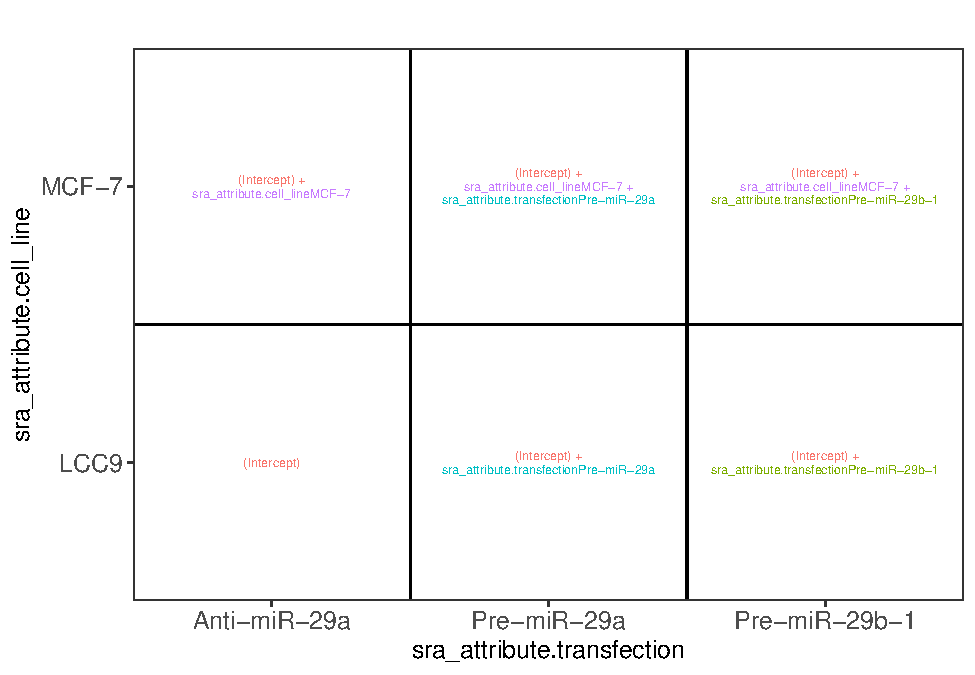
\includegraphics{Proyecto_RNAseq_files/figure-latex/unnamed-chunk-11-1.pdf}

sra\_attribute.cell\_lineMCF-7: Este coeficiente es la diferencia entre
la línea celular sensible al tratamiento (MCF-7), contra la línea
celular resistente al tratamiento (LCC9), cuando la transfección se
mantiene constante. De modo que, representa la diferencia en la
respuesta entre la línea celular MCF-7 y la línea celular LCC9.

\subsection{Expresión diferencial}\label{expresiuxf3n-diferencial}

\begin{Shaded}
\begin{Highlighting}[]
\CommentTok{\# Convertir los datos de conteo a valores log2 y ajusta las varianzas para }
\CommentTok{\# hacerlos aptos para un análisis lineal }

\NormalTok{vGene }\OtherTok{\textless{}{-}} \FunctionTok{voom}\NormalTok{(dge, mod, }\AttributeTok{plot =} \ConstantTok{TRUE}\NormalTok{)}
\end{Highlighting}
\end{Shaded}

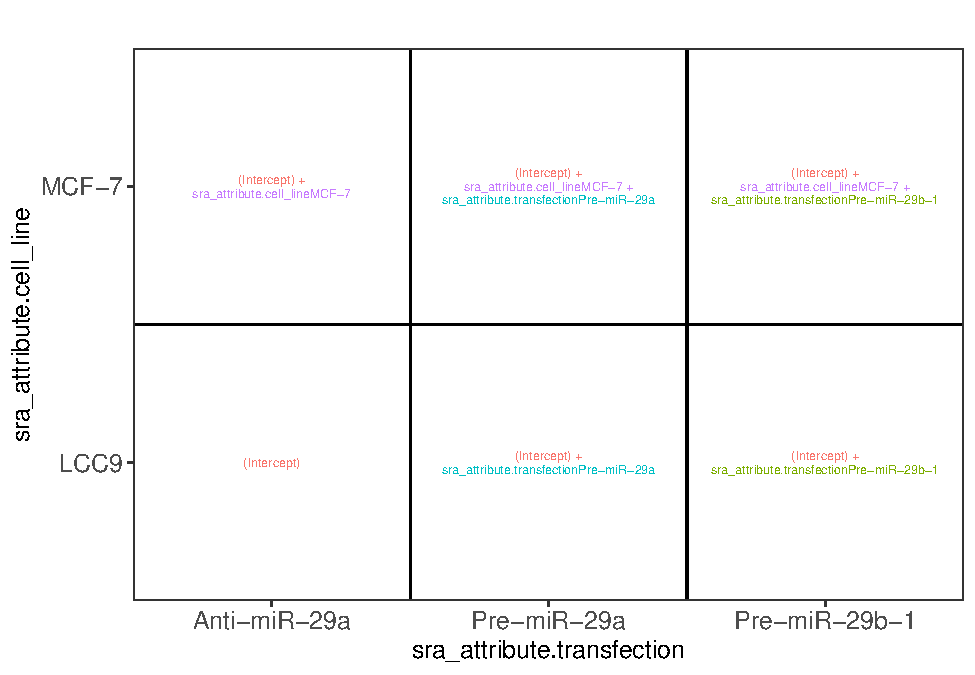
\includegraphics{Proyecto_RNAseq_files/figure-latex/unnamed-chunk-12-1.pdf}

El método voom estima la relación media-varianza de los recuentos
logarítmicos, genera un peso de precisión para cada observación y los
ingresa en el flujo de trabajo del análisis bayesiano empírico de Limma.
Por lo tanto, este gráfico muestra la relación entre la media y la
varianza de los datos de expresión génica en escala log2. En el eje X se
observa la expresión promedio de los genes, mientras que el eje Y
representa la raíz cuadrada de la desviación estándar. Los genes con
baja expresión presentan mayor dispersión, mientras que a niveles altos
de expresión la varianza disminuye y se estabiliza. (Law et al. 2014)

\begin{Shaded}
\begin{Highlighting}[]
\CommentTok{\# Ajuste del modelo lineal y cálculo de estadísticas empíricas de Bayes}
\NormalTok{eb\_results }\OtherTok{\textless{}{-}} \FunctionTok{eBayes}\NormalTok{(}\FunctionTok{lmFit}\NormalTok{(vGene))}


\CommentTok{\# Extraer la tabla de genes diferencialmente expresados.}
\NormalTok{de\_results }\OtherTok{\textless{}{-}} \FunctionTok{topTable}\NormalTok{(}
\NormalTok{    eb\_results,}
    \AttributeTok{coef =} \DecValTok{2}\NormalTok{, }\CommentTok{\# Se refiere al coeficiente del segundo término en el modelo}
    \AttributeTok{number =} \FunctionTok{nrow}\NormalTok{(rse\_gene\_SRP075398),}
    \AttributeTok{sort.by =} \StringTok{"none"}
\NormalTok{)}

\CommentTok{\# Dimensiones y vista preliminar de los resultados}
\FunctionTok{dim}\NormalTok{(de\_results)}
\end{Highlighting}
\end{Shaded}

\begin{verbatim}
## [1] 23741    16
\end{verbatim}

\begin{Shaded}
\begin{Highlighting}[]
\FunctionTok{head}\NormalTok{(de\_results)}
\end{Highlighting}
\end{Shaded}

\begin{verbatim}
##                   source type bp_length phase           gene_id
## ENSG00000223972.5 HAVANA gene      1735    NA ENSG00000223972.5
## ENSG00000227232.5 HAVANA gene      1351    NA ENSG00000227232.5
## ENSG00000238009.6 HAVANA gene      3726    NA ENSG00000238009.6
## ENSG00000233750.3 HAVANA gene      3812    NA ENSG00000233750.3
## ENSG00000268903.1 HAVANA gene       755    NA ENSG00000268903.1
## ENSG00000269981.1 HAVANA gene       284    NA ENSG00000269981.1
##                                            gene_type     gene_name level
## ENSG00000223972.5 transcribed_unprocessed_pseudogene       DDX11L1     2
## ENSG00000227232.5             unprocessed_pseudogene        WASH7P     2
## ENSG00000238009.6                            lincRNA  RP11-34P13.7     2
## ENSG00000233750.3               processed_pseudogene        CICP27     1
## ENSG00000268903.1               processed_pseudogene RP11-34P13.15     2
## ENSG00000269981.1               processed_pseudogene RP11-34P13.16     2
##                            havana_gene               tag       logFC    AveExpr
## ENSG00000223972.5 OTTHUMG00000000961.2              <NA> -1.57964773 -0.7349755
## ENSG00000227232.5 OTTHUMG00000000958.1              <NA> -0.65730720  2.4021094
## ENSG00000238009.6 OTTHUMG00000001096.2 overlapping_locus  0.50892797 -0.5758187
## ENSG00000233750.3 OTTHUMG00000001257.3    pseudo_consens  0.07505824 -2.5024602
## ENSG00000268903.1 OTTHUMG00000182518.2              <NA> -2.26677866 -2.9392186
## ENSG00000269981.1 OTTHUMG00000182738.2              <NA> -0.20655991 -1.1726322
##                            t      P.Value    adj.P.Val         B
## ENSG00000223972.5 -9.0583130 5.502604e-08 1.724585e-07  8.293369
## ENSG00000227232.5 -4.2492998 5.203366e-04 8.224575e-04 -1.699547
## ENSG00000238009.6  3.2989311 4.153389e-03 5.833271e-03 -3.230385
## ENSG00000233750.3  0.2097501 8.363087e-01 8.516989e-01 -7.250773
## ENSG00000268903.1 -4.8120051 1.545050e-04 2.624197e-04  0.559485
## ENSG00000269981.1 -0.8707765 3.957782e-01 4.289509e-01 -7.156075
\end{verbatim}

El coeficiente 2 (sra\_attribute.cell\_lineMCF-7) evalúa la expresión
diferencial entre las líneas celulares MCF-7 y LCC9, lo que podría
permitir identificar genes relacionados con la resistencia a la terapia
endocrina.

\begin{Shaded}
\begin{Highlighting}[]
\CommentTok{\# Genes diferencialmente expresados con FDR \textless{} 5\%}
\FunctionTok{table}\NormalTok{(de\_results}\SpecialCharTok{$}\NormalTok{adj.P.Val }\SpecialCharTok{\textless{}} \FloatTok{0.05}\NormalTok{)}
\end{Highlighting}
\end{Shaded}

\begin{verbatim}
## 
## FALSE  TRUE 
##  4642 19099
\end{verbatim}

\begin{Shaded}
\begin{Highlighting}[]
\CommentTok{\# Visualizar los resultados estadísticos}

\FunctionTok{plotMA}\NormalTok{(eb\_results, }\AttributeTok{coef =} \DecValTok{2}\NormalTok{)}
\end{Highlighting}
\end{Shaded}

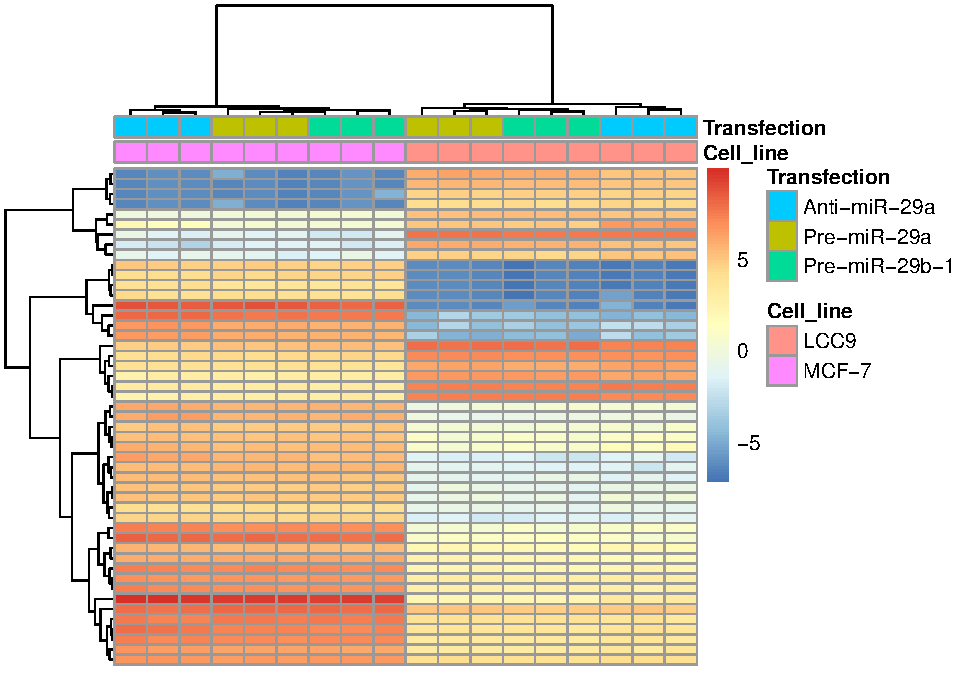
\includegraphics{Proyecto_RNAseq_files/figure-latex/unnamed-chunk-14-1.pdf}

El gráfico generado por la función plotMA() en el análisis de expresión
diferencial muestra los resultados estadísticos del contraste entre las
líneas celulares MCF-7 y LCC9. En este tipo de gráfico, el eje X
representa la expresión promedio en escala logarítmica para cada gen,
mientras que el eje Y muestra el cambio logarítmico en la expresión
(log2 fold-change) asociado al coeficiente 2 del modelo.La línea
horizontal en y = 0 representa genes sin cambios significativos en su
expresión.

\begin{Shaded}
\begin{Highlighting}[]
\FunctionTok{volcanoplot}\NormalTok{(eb\_results, }\AttributeTok{coef =} \DecValTok{2}\NormalTok{, }\AttributeTok{highlight =} \DecValTok{3}\NormalTok{, }\AttributeTok{names =}\NormalTok{ de\_results}\SpecialCharTok{$}\NormalTok{gene\_name)}
\end{Highlighting}
\end{Shaded}

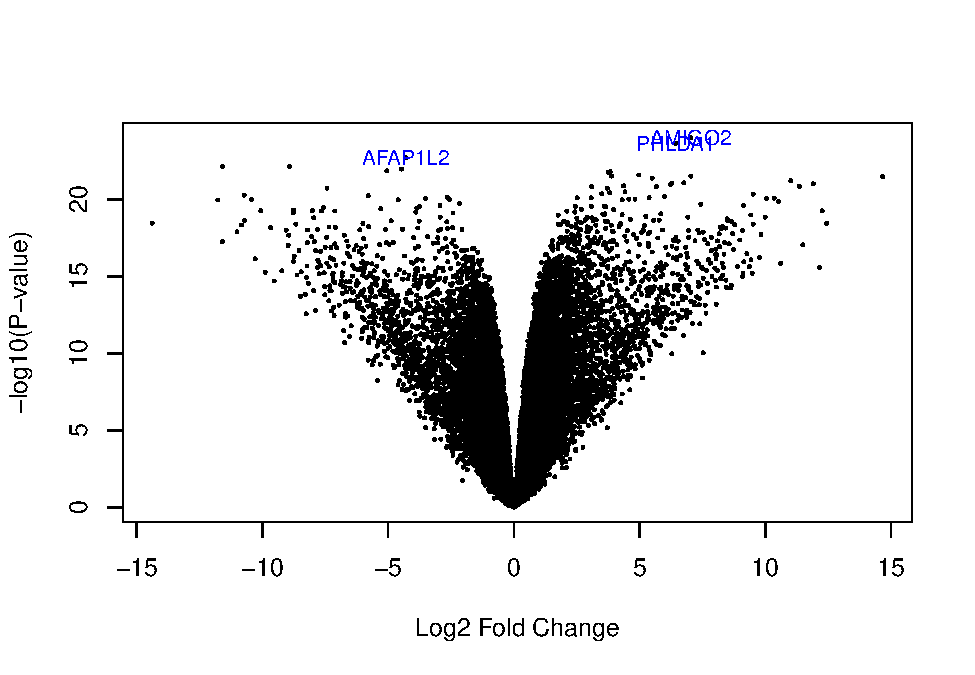
\includegraphics{Proyecto_RNAseq_files/figure-latex/unnamed-chunk-15-1.pdf}

\begin{Shaded}
\begin{Highlighting}[]
\CommentTok{\# Información de los 3 genes más significativos }
\NormalTok{de\_results[de\_results}\SpecialCharTok{$}\NormalTok{gene\_name }\SpecialCharTok{\%in\%} \FunctionTok{c}\NormalTok{(}\StringTok{"AMIGO2"}\NormalTok{, }\StringTok{"AFAP1L2"}\NormalTok{, }\StringTok{"PHLDA1"}\NormalTok{), ]}
\end{Highlighting}
\end{Shaded}

\begin{verbatim}
##                    source type bp_length phase            gene_id
## ENSG00000169129.14 HAVANA gene      5789    NA ENSG00000169129.14
## ENSG00000139211.6  HAVANA gene      3956    NA  ENSG00000139211.6
## ENSG00000139289.13 HAVANA gene      8069    NA ENSG00000139289.13
##                         gene_type gene_name level          havana_gene  tag
## ENSG00000169129.14 protein_coding   AFAP1L2     2 OTTHUMG00000019086.3 <NA>
## ENSG00000139211.6  protein_coding    AMIGO2     2 OTTHUMG00000169616.1 <NA>
## ENSG00000139289.13 protein_coding    PHLDA1     2 OTTHUMG00000169783.2 <NA>
##                        logFC  AveExpr         t      P.Value    adj.P.Val
## ENSG00000169129.14 -4.302232 5.257918 -77.07393 1.991303e-23 1.575851e-19
## ENSG00000139211.6   7.038259 6.044177  91.73069 9.814316e-25 2.330017e-20
## ENSG00000139289.13  6.438081 3.881338  87.38040 2.274059e-24 2.699422e-20
##                           B
## ENSG00000169129.14 43.77924
## ENSG00000139211.6  46.45332
## ENSG00000139289.13 45.06009
\end{verbatim}

\href{https://www.genecards.org/cgi-bin/carddisp.pl?gene=AMIGO2&keywords=AMIGO2}{AMIGO2
en GeneCards}

\href{https://www.genecards.org/cgi-bin/carddisp.pl?gene=AFAP1L2&keywords=AFAP1L2}{AFAP1L2
en GeneCards}

\href{https://www.genecards.org/cgi-bin/carddisp.pl?gene=PHLDA1&keywords=PHLDA1}{PHLDA1
en GeneCards}

En el volcanoplot creado los genes más significativos se muestran en la
parte superior. Cada punto del gráfico representa un gen. Las
diferencias de log 2 entre los grupos se representan en el eje x y las
diferencias de log 10 en el valor p se representan en el eje y. Los
genes cuya expresión disminuye se ubican a la izquierda del cero en el
eje x, mientras que los genes cuya expresión aumenta se ilustran a la
derecha del cero. Entonces, el gráfico muestra genes con aumento de
expresión en MCF-7 (sensible) a la derecha (en comparación con LCC9), y
genes con disminución de expresión en MCF-7 a la izquierda (en
comparación con LCC9).

\subsection{Visualizar genes DE}\label{visualizar-genes-de}

\begin{Shaded}
\begin{Highlighting}[]
\CommentTok{\# Revisar los top 50 genes diferencialmente expresados}

\CommentTok{\# Extraer valores de los genes de interés}
\NormalTok{exprs\_heatmap }\OtherTok{\textless{}{-}}\NormalTok{ vGene}\SpecialCharTok{$}\NormalTok{E[}\FunctionTok{rank}\NormalTok{(de\_results}\SpecialCharTok{$}\NormalTok{adj.P.Val) }\SpecialCharTok{\textless{}=} \DecValTok{50}\NormalTok{, ]}

\CommentTok{\# Crear una tabla con información de las muestras y con nombres de columnas más amigables}
\NormalTok{df }\OtherTok{\textless{}{-}} \FunctionTok{as.data.frame}\NormalTok{(}\FunctionTok{colData}\NormalTok{(rse\_gene\_SRP075398)[, }\FunctionTok{c}\NormalTok{(}\StringTok{"sra\_attribute.cell\_line"}\NormalTok{,}
                                              \StringTok{"sra\_attribute.transfection"}\NormalTok{)])}

\FunctionTok{colnames}\NormalTok{(df) }\OtherTok{\textless{}{-}} \FunctionTok{c}\NormalTok{(}\StringTok{"Cell\_line"}\NormalTok{, }\StringTok{"Transfection"}\NormalTok{)}
\end{Highlighting}
\end{Shaded}

\begin{Shaded}
\begin{Highlighting}[]
\DocumentationTok{\#\# Guardemos los IDs de nuestros 50 genes}
\NormalTok{nombres\_originales }\OtherTok{\textless{}{-}} \FunctionTok{rownames}\NormalTok{(exprs\_heatmap)}

\DocumentationTok{\#\# Con match() podemos encontrar cual es cual}
\FunctionTok{rownames}\NormalTok{(exprs\_heatmap) }\OtherTok{\textless{}{-}} \FunctionTok{rowRanges}\NormalTok{(rse\_gene\_SRP075398)}\SpecialCharTok{$}\NormalTok{gene\_name[}
    \FunctionTok{match}\NormalTok{(}\FunctionTok{rownames}\NormalTok{(exprs\_heatmap), }\FunctionTok{rowRanges}\NormalTok{(rse\_gene\_SRP075398)}\SpecialCharTok{$}\NormalTok{gene\_id)}
\NormalTok{]}

\DocumentationTok{\#\# Guardar la imagen en un PDF largo para poder ver los nombres de los genes}
\FunctionTok{pdf}\NormalTok{(}\StringTok{"pheatmap\_con\_nombres.pdf"}\NormalTok{, }\AttributeTok{height =} \DecValTok{16}\NormalTok{, }\AttributeTok{useDingbats =} \ConstantTok{FALSE}\NormalTok{)}
\FunctionTok{pheatmap}\NormalTok{(}
\NormalTok{    exprs\_heatmap,}
    \AttributeTok{cluster\_rows =} \ConstantTok{TRUE}\NormalTok{,}
    \AttributeTok{cluster\_cols =} \ConstantTok{TRUE}\NormalTok{,}
    \AttributeTok{show\_rownames =} \ConstantTok{TRUE}\NormalTok{,}
    \AttributeTok{show\_colnames =} \ConstantTok{FALSE}\NormalTok{,}
    \AttributeTok{annotation\_col =}\NormalTok{ df,}
    \AttributeTok{fontsize\_row =} \DecValTok{6}\NormalTok{,}
\NormalTok{)}
\end{Highlighting}
\end{Shaded}

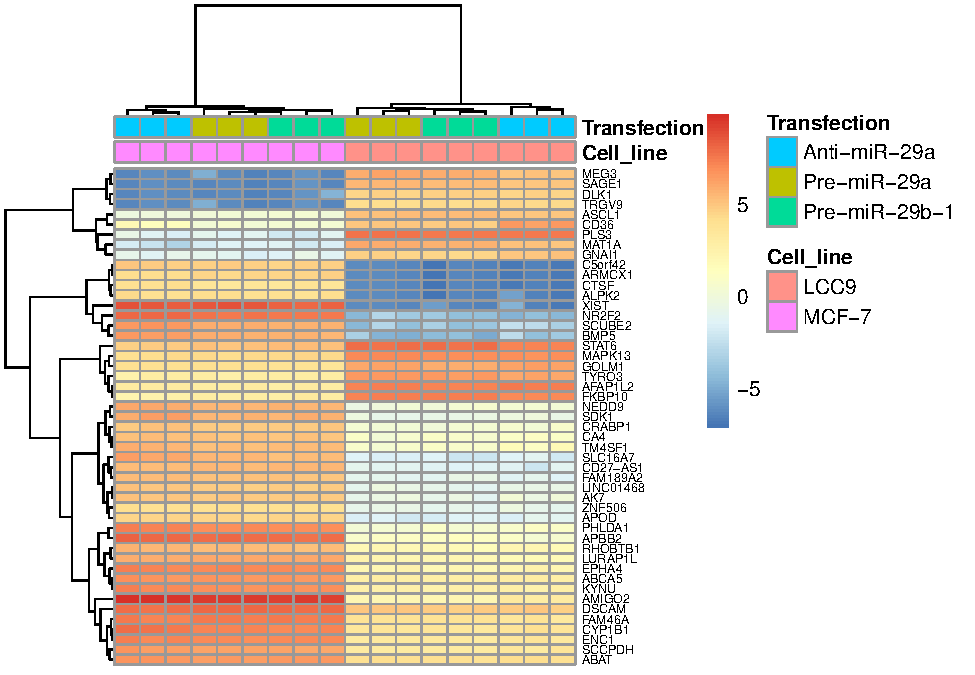
\includegraphics{Proyecto_RNAseq_files/figure-latex/unnamed-chunk-17-1.pdf}

\begin{Shaded}
\begin{Highlighting}[]
\FunctionTok{dev.off}\NormalTok{()}
\end{Highlighting}
\end{Shaded}

\begin{verbatim}
## pdf 
##   3
\end{verbatim}

El heatmap muestra patrones de expresión génica distintos entre las
líneas celulares LCC9 (resistente al tratamiento) y MCF-7 (sensible al
tratamiento) en respuesta a diferentes transfecciones. En general, se
observa una diferencia en la expresión de genes entre ambas líneas
celulares. Con respecto a, genes específicos como AMIGO2 se observa una
expresión más alta en las células MCF-7 en comparación con las células
LCC9, con todos los tipos de miRNAs usados para la transfección. Otros
genes como AFAP1L2, PLS3, STAT6, FKBP10 también muestran patrones de
expresión interesantes, con niveles más altos en las células LCC9 en
comparación con las células MCF-7, especialmente en las muestras
transfectadas con Pre-miR-29a y Pre-miR-29b-1.

Por otro lado, PHLDA1 no muestra diferencias tan marcadas en su
expresión entre las dos líneas celulares, aunque parece tener una
expresión ligeramente más alta en las células MCF-7 en comparación con
las células LCC9.

\begin{Shaded}
\begin{Highlighting}[]
\CommentTok{\# MDS (multidimensional scaling)}

\DocumentationTok{\#\# Convertir los grupos de Cell\_line a colores}
\NormalTok{col.group }\OtherTok{\textless{}{-}}\NormalTok{ df}\SpecialCharTok{$}\NormalTok{Cell\_line}
\FunctionTok{levels}\NormalTok{(col.group) }\OtherTok{\textless{}{-}} \FunctionTok{brewer.pal}\NormalTok{(}\FunctionTok{nlevels}\NormalTok{(col.group), }\StringTok{"Set2"}\NormalTok{)}
\end{Highlighting}
\end{Shaded}

\begin{verbatim}
## Warning in brewer.pal(nlevels(col.group), "Set2"): minimal value for n is 3, returning requested palette with 3 different levels
\end{verbatim}

\begin{Shaded}
\begin{Highlighting}[]
\NormalTok{col.group }\OtherTok{\textless{}{-}} \FunctionTok{as.character}\NormalTok{(col.group)}

\DocumentationTok{\#\# MDS por grupos de Cell\_line}
\FunctionTok{plotMDS}\NormalTok{(vGene}\SpecialCharTok{$}\NormalTok{E, }\AttributeTok{labels =}\NormalTok{ df}\SpecialCharTok{$}\NormalTok{Cell\_line, }\AttributeTok{col =}\NormalTok{ col.group)}
\end{Highlighting}
\end{Shaded}

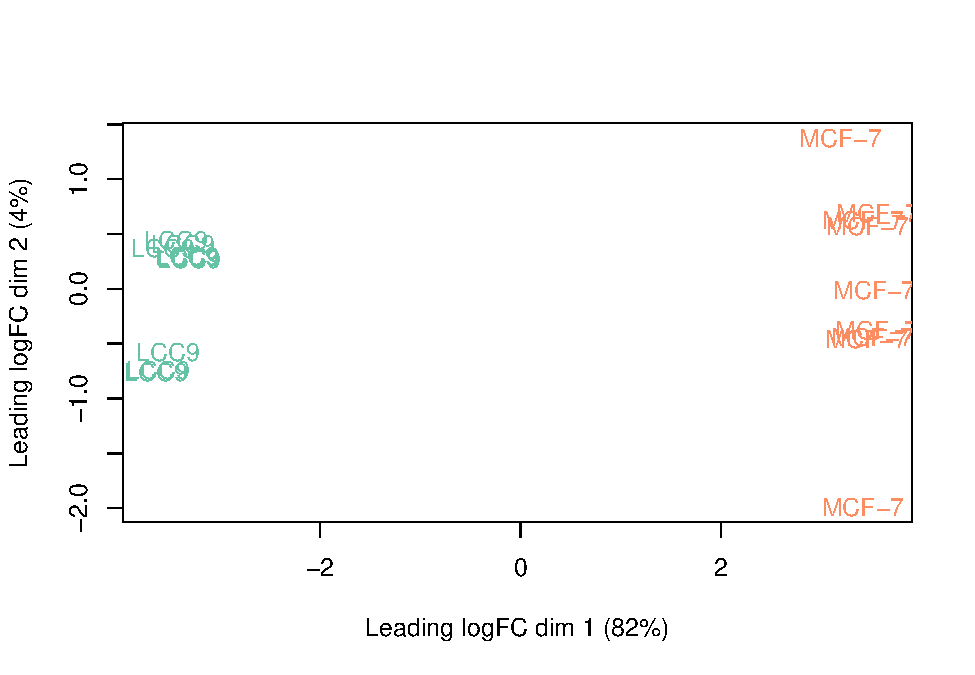
\includegraphics{Proyecto_RNAseq_files/figure-latex/unnamed-chunk-18-1.pdf}

Este gráfico evalúa si las muestras se agrupan según la variable
Cell\_line, la separación clara entre MCF-7 y LCC9 indica que hay
diferencias notables en la expresión génica entre estas líneas
celulares. Esto sugiere que LCC9 y MCF-7 tienen perfiles de expresión
distintos, lo que podría estar influenciado por la transfección con
miR-29a/b. Por lo tanto, es posible que los genes regulados por
miR-29a/b sean clave en la resistencia a la terapia endocrina.

\begin{Shaded}
\begin{Highlighting}[]
\DocumentationTok{\#\# Convertir Transfection a colores}
\NormalTok{col.group }\OtherTok{\textless{}{-}}\NormalTok{ df}\SpecialCharTok{$}\NormalTok{Transfection}
\NormalTok{df}\SpecialCharTok{$}\NormalTok{Transfection }\OtherTok{\textless{}{-}} \FunctionTok{as.factor}\NormalTok{(df}\SpecialCharTok{$}\NormalTok{Transfection) }\CommentTok{\# Asegúrate de que sea un factor}
\NormalTok{colors }\OtherTok{\textless{}{-}} \FunctionTok{brewer.pal}\NormalTok{(}\FunctionTok{nlevels}\NormalTok{(df}\SpecialCharTok{$}\NormalTok{Transfection), }\StringTok{"Set2"}\NormalTok{) }\CommentTok{\# Generar paleta de colores}
\FunctionTok{levels}\NormalTok{(col.group) }\OtherTok{\textless{}{-}}\NormalTok{ colors }\CommentTok{\# Asignar colores a los niveles}
\NormalTok{col.group }\OtherTok{\textless{}{-}} \FunctionTok{as.character}\NormalTok{(col.group) }\CommentTok{\# Convertir a vector de caracteres}

\DocumentationTok{\#\# MDS por grupos de Transfection}
\FunctionTok{plotMDS}\NormalTok{(vGene}\SpecialCharTok{$}\NormalTok{E, }\AttributeTok{labels =}\NormalTok{ df}\SpecialCharTok{$}\NormalTok{Transfection, }\AttributeTok{col =}\NormalTok{ col.group, }
        \AttributeTok{main =} \StringTok{"MDS Plot by Transfection"}\NormalTok{, }\AttributeTok{pch =} \DecValTok{16}\NormalTok{)}

\DocumentationTok{\#\# Agregar leyenda}
\FunctionTok{legend}\NormalTok{(}\StringTok{"center"}\NormalTok{, }\AttributeTok{legend =} \FunctionTok{levels}\NormalTok{(df}\SpecialCharTok{$}\NormalTok{Transfection), }\AttributeTok{fill =} \FunctionTok{unique}\NormalTok{(col.group),}
       \AttributeTok{title =} \StringTok{"Transfection Groups"}\NormalTok{)}
\end{Highlighting}
\end{Shaded}

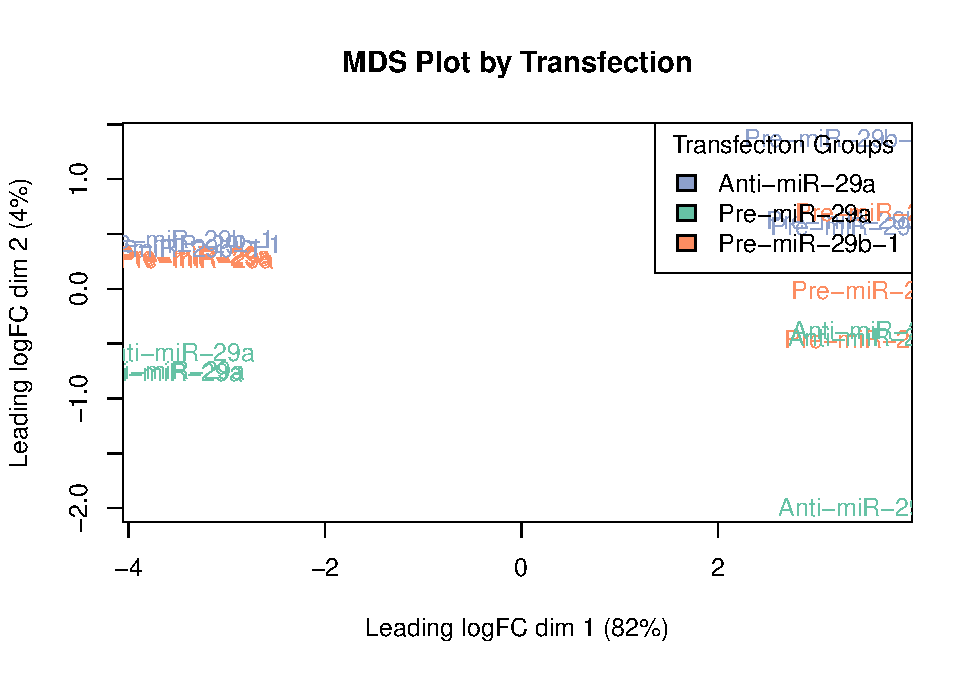
\includegraphics{Proyecto_RNAseq_files/figure-latex/unnamed-chunk-19-1.pdf}

El gráfico MDS muestra una cierta separación entre los grupos de
transfección, donde Anti-miR-29a presenta un perfil distinto en
comparación con Pre-miR-29a y Pre-miR-29b-1, que comparten similitudes
pero aún muestran cierta dispersión. La dimensión principal (logFC dim
1) captura la mayor variabilidad en la expresión génica, sugiriendo que
la transfección tiene un impacto significativo.

\subsection{Conclusión}\label{conclusiuxf3n}

El análisis de expresión diferencial realizado en este proyecto permitió
identificar genes relacionados con la resistencia a la terapia endocrina
en cáncer de mama. A través de diversas visualizaciones, se evidenciaron
diferencias significativas en los perfiles de expresión entre las líneas
celulares MCF-7 (sensibles) y LCC9 (resistentes). El heatmap mostró
patrones distintivos de expresión génica entre ambas líneas celulares,
destacando genes como AMIGO2 con mayor expresión en MCF-7, mientras que
AFAP1L2, PLS3, STAT6 y FKBP10 presentaron niveles más altos en LCC9.

Además, los paquetes empleados en este estudio, son herramientas
bioinformpaticas muy útiles que permiten llevar a cabo un protocolo
estándar para el análisis de expresión diferencial que incluye:
procesamiento de datos, filtrado de genes, normalización, construcción
de modelos y pruebas estadísticas. Por lo que, el conocimiento de este
flujo de trabajo es fundamental para cualquier investigador que busca
comprender mecanismos moleculares o desarrollar nuevas estrategias
terapéuticas.

\subsection*{Referencias}\label{referencias}
\addcontentsline{toc}{subsection}{Referencias}

\phantomsection\label{refs}
\begin{CSLReferences}{1}{0}
\bibitem[\citeproctext]{ref-Law2014}
Law, Charity W., Yunshun Chen, Wei Shi, and Gordon K. Smyth. 2014.
{``Voom: Precision Weights Unlock Linear Model Analysis Tools for
RNA-Seq Read Counts.''} \emph{Genome Biology} 15 (February).
\url{https://doi.org/10.1186/gb-2014-15-2-r29}.

\bibitem[\citeproctext]{ref-Muluhngwi2021}
Muluhngwi, Penn, and Carolyn M. Klinge. 2021. {``Identification and
Roles of Mir-29b-1-3p and Mir29a-3p-Regulated and Non-Regulated Lncrnas
in Endocrine-Sensitive and Resistant Breast Cancer Cells.''}
\emph{Cancers} 13 (July). \url{https://doi.org/10.3390/cancers13143530}.

\end{CSLReferences}

\end{document}
